% Results of the sweep. Every value below is a macro from sections/generated_numbers.tex,
% generated from the run's summary and provenance files by scripts/paper/fill_v060_numbers.py.
% No number is typed here.

\section{Results}\label{sec:results}

\subsection{Pre-registered hypotheses and criteria}\label{subsec:prereg}

The hypotheses, their criteria and the analysis plan were fixed in a pre-registration that is
released with the code (\S\ref{sec:reproducibility}). It was amended four times before any data
from this sweep existed, and twice more after the outcome was known: once changing only the
title and one term, and once changing the title again and recording that the exploratory
analyses of \S\ref{subsec:exploratory} were added after the outcome. Neither changes a
hypothesis, a threshold, an estimator or an outcome. Table~\ref{tab:amendments} lists the amendments, and the run's provenance record
identifies the revision of the pre-registration in force. Table~\ref{tab:gates} states the five
hypotheses and their criteria. Each criterion is reported as supported, not supported or, when the
data do not allow it to be computed, as not evaluable, with the reason; a criterion that cannot
be evaluated is never counted as not supported, and the tally is always
stated out of five. In the text we refer to the hypotheses by what they claim: the two
\emph{attainable-error} hypotheses, one per screen; the \emph{backbone-choice} hypothesis; the
\emph{trace-feature ranking} hypothesis; and the \emph{cross-dataset transfer} hypothesis.
Bootstrap confidence intervals (CIs) are 95\% percentile intervals over \emph{tasks}, with $B=10\,000$
resamples from a generator seeded with 2026. In summary, \resGateSummary.

The five criteria are of three kinds, and the tally should be read with that in mind. The two
attainable-error hypotheses are feasibility checks on an oracle quantity, the best
configuration selected on the same data it is scored on (\S\ref{subsec:oracle}). The backbone-choice hypothesis checks that a design lever was exercised. Only the
ranking and transfer hypotheses bear on the title question, and of those two one is supported
and one is not. Each criterion is a threshold on a point estimate. No error rate spanning the
five was pre-registered and no power analysis was made; the only quantified false-positive rate
is that of the ranking criterion (\S\ref{sec:tdi-real}).

\begin{table}[htp]
\footnotesize
\centering
\begin{tabular}{p{0.03\linewidth}p{0.09\linewidth}p{0.1\linewidth}p{0.17\linewidth}p{0.45\linewidth}}
\toprule
No. & Version tag & Locked (UTC) & Lock commit(s) & Change \\
\midrule
1 & \resAmendOneVersion$^{\dagger}$ & \resAmendOneDate & \texttt{\resAmendOneCommit} & \resAmendOneChange \\
2 & \texttt{\resAmendTwoVersion} & \resAmendTwoDate & \texttt{\resAmendTwoCommit} & \resAmendTwoChange \\
3 & \texttt{\resAmendThreeVersion} & \resAmendThreeDate & \texttt{\resAmendThreeCommit} & \resAmendThreeChange \\
4 & \texttt{\resAmendFourVersion} & \resAmendFourDate & \texttt{\resAmendFourCommit} & \resAmendFourChange \\
\midrule
5 & \texttt{\resAmendFiveVersion}$^{\ddagger}$ & \resAmendFiveDate & \texttt{\resAmendFiveCommit} & \resAmendFiveChange \\
6 & \texttt{\resAmendSixVersion}$^{\ddagger}$ & \resAmendSixDate & \texttt{\resAmendSixCommit} & \resAmendSixChange \\
\bottomrule
\end{tabular}
\caption{The six amendments to the pre-registration, numbered in order. For each, the table
gives the version tag of the pre-registration in the released repository, the date on which
the amendment was locked, the repository commit or commits that locked its text (the lock
commits), and what it changed. Amendments 1--4 were each locked before any data from this
sweep existed. $^{\ddagger}$Amendments 5 and 6 were locked \emph{after} the outcome was known;
the fifth changes the title and one term only, the sixth changes the title again and records
the exploratory analyses added after the outcome, and no run exists under either.
$^{\dagger}$The first amendment predates the
version tags, so it has none; the run was made under the fourth amendment's tag. For the fourth
amendment, \resAmendFourNote. Dates and commits are taken from the repository history and
checked against it automatically.}
\label{tab:amendments}
\end{table}

\begin{table}[htp]
\small
\centering
\begin{tabular}{p{0.43\linewidth}p{0.24\linewidth}p{0.24\linewidth}}
\toprule
Hypothesis & Criterion & Outcome \\
\midrule
\emph{Attainable error on Adamson.} The trainer sweep attains low held-out error on the
  Adamson tasks.
  & The median over tasks of the lowest MSD is below $\resHOneThreshold$.
  & \resHOneVerdict{} (median \resHOneMedian) \\
\addlinespace
\emph{Attainable error on Norman.} The trainer sweep attains low held-out error on the
  Norman tasks.
  & The median over tasks of the lowest MSD is below $\resHTwoThreshold$.
  & \resHTwoVerdict{} (median \resHTwoMedian) \\
\addlinespace
\emph{Backbone choice.} The Architect uses its choice of backbone: the backbones it states,
  pooled over all its LLM-sourced steps across tasks, seeds and rounds, are varied.
  & The Shannon entropy of the stated backbone is at least $0.5$ nats.
  & \resHThreeVerdict{} (\resHThreeEntropy{} nats) \\
\addlinespace
\emph{Trace-feature ranking.} A feature of the trace ($\mathrm{ACE}_{\mathrm{norm}}$,
  $1-\Delta C$ or $\mathrm{TDI}_{\mathrm{lifecycle}}$) ranks tasks by held-out error.
  & Spearman's $\rho$ exceeds $0.5$ in at least one of the six within-dataset tests.
  & \resHFourVerdict{} (\resHFourNPassing{} of \resHFourNTests{} tests) \\
\addlinespace
\emph{Cross-dataset transfer.} $\mathrm{TDI}_{\mathrm{lifecycle}}$ with weights fitted by
  ridge regression on the Adamson tasks ranks the Norman tasks by held-out error.
  & Spearman's $\rho$ on the Norman tasks exceeds $\resHFiveThreshold$.
  & \resHFiveVerdict{} ($\rho=\resHFiveRho$) \\
\bottomrule
\end{tabular}
\caption{The five pre-registered hypotheses, each named as it is in the text, with its
criterion and outcome. The outcome reads \emph{supported} when the
criterion is met, \emph{not supported} when it is not, and \emph{not evaluable} when the data do
not allow the test. Tally out of \resTallyOut: supported \resTallyPass, not supported
\resTallyFail, not evaluable \resTallyUneval. Held-out error is the mean squared deviation
(MSD) on the evaluation genes (\S\ref{subsec:eval}); the lowest MSD of the trainer sweep is an
oracle quantity (\S\ref{subsec:oracle}). $\mathrm{ACE}_{\mathrm{norm}}$ is the normalised
entropy of the agents' final-round confidences, $1-\Delta C$ is one minus the change in their
mean confidence from the first round to the last, and $\mathrm{TDI}_{\mathrm{lifecycle}}$ is
the weighted composite of the two (\S\ref{sec:tdi-real}); $\rho$ is Spearman's rank
correlation across tasks. The estimators are given in the subsections that follow
and in the pre-registration.}
\label{tab:gates}
\end{table}

\subsection{Lowest error reached by the trainer sweep}\label{subsec:h12}

The two attainable-error hypotheses are tested, per task, with the minimum MSD on the top-$20$
evaluation genes over the \resNDistinctConfigs{} distinct trainer configurations
(\resNTrainerRecordsPerTask{} records per task). Because this minimum is selected on the data it
is scored on, it is an oracle (\S\ref{subsec:oracle}). The criterion is the median of the
minimum over the tasks of each dataset. The evaluation genes are fixed per task, for all
\resEvalGeneTasks{} tasks, and the agentic lifecycle is scored on the same genes, as amended
before data collection (Table~\ref{tab:amendments}); the trainer's and the lifecycle's gene
lists differ on \resEvalGeneMismatch{} tasks. Table~\ref{tab:headline-msd} gives the
distribution of the per-task minimum in each dataset.

\begin{table}[htp]
\small
\centering
\resizebox{\linewidth}{!}{%
\begin{tabular}{lllllll}
\toprule
Dataset & $n$ & Median & IQR & Maximum & Fraction over criterion & 95\% CI of the median \\
\midrule
Adamson 2016 & \resHOneN & \resHOneMedian & [\resHOneIQRLo, \resHOneIQRHi] & \resHOneMax & \resHOneFracOver & [\resHOneCILo, \resHOneCIHi] \\
Norman 2019 & \resHTwoN & \resHTwoMedian & [\resHTwoIQRLo, \resHTwoIQRHi] & \resHTwoMax & \resHTwoFracOver & [\resHTwoCILo, \resHTwoCIHi] \\
\quad singletons & \resHTwoSingletonN & \resHTwoSingletonMedian & [\resHTwoSingletonIQRLo, \resHTwoSingletonIQRHi] & \resHTwoSingletonMax & \resHTwoSingletonFracOver & --- \\
\quad doublets & \resHTwoDoubletN & \resHTwoDoubletMedian & [\resHTwoDoubletIQRLo, \resHTwoDoubletIQRHi] & \resHTwoDoubletMax & \resHTwoDoubletFracOver & --- \\
\bottomrule
\end{tabular}}
\caption{The lowest mean squared deviation (MSD) that the trainer sweep reaches on the
top-$20$ evaluation genes of each task, summarised over the $n$ tasks of each dataset. The
minimum is taken over the distinct configurations and selected on the same data it is scored
on, so it is an oracle quantity (\S\ref{subsec:oracle}). IQR is the interquartile range, and
CI the bootstrap confidence interval over tasks. The criteria are an Adamson median below
$\resHOneThreshold$ (\resHOneVerdict) and a Norman median below $\resHTwoThreshold$
(\resHTwoVerdict). Singletons and doublets are the single-gene and two-gene perturbations of
Norman. Bootstrap CIs
are not computed per stratum. The median of the Norman doublet stratum
(\resHTwoDoubletMedian) lies above the criterion; the criterion is the median over all
$\resHTwoN$ Norman tasks.}
\label{tab:headline-msd}
\end{table}

\subsection{Does the Architect use its choice of backbone?}\label{subsec:h3}

The backbone-choice hypothesis is tested with the plug-in Shannon entropy, in nats, of the
backbone the Architect \emph{stated}, pooled over all LLM-sourced Architect steps across tasks,
seeds and rounds. It is a statement about the
pool, not about any task, seed or round. With three backbones on the menu the entropy cannot
exceed $\ln 3=\resHThreeCeiling$; the use of the stated backbone and of a fixed menu was settled
before data collection (Table~\ref{tab:amendments}). Of \resHThreeNSteps{} Architect steps,
\resHThreeNCounted{} were counted: \resHThreeNMissingStated{} stated no backbone and
\resHThreeNOffMenu{} stated one that is not on the menu. The Architect stated \textsc{linear}
\resHThreePickLinear{} times, \textsc{mlp} \resHThreePickMlp{} times and the transformer
\resHThreePickScgpt{} times, an entropy of \resHThreeEntropy{} nats, so the hypothesis is
\resHThreeVerdict. Executed-pick counts, reported alongside and not entering the criterion, are
\textsc{linear} \resHThreeExecPickLinear, \textsc{mlp} \resHThreeExecPickMlp{} and the transformer
\resHThreeExecPickScgpt{} (entropy \resHThreeEntropyExecuted{} nats, with
\resHThreeNMissingExecuted{} steps lacking an executed backbone). The executed backbone
equalled the stated one on every step; the count of steps where they differ is
\resHThreeExecNeStated. As a descriptive check, the Miller--Madow bias-corrected entropy
$H+(K-1)/(2M)$, with $K=\resHThreeMenuSize$ backbones and $M=\resHThreeNCounted$ counted steps, is
\resHThreeMillerMadowNats{} nats; the criterion uses the plug-in value, as pre-registered. The
correction is pre-registered for breakdowns with $M<50$; the smallest breakdown here, by serving
model, has $M=\resHThreeSmallestBreakdownN$, so the correction is \resHThreeMillerMadow. All
Architect steps were served by one model, Claude Haiku 4.5 (\resRosterHaiku;
\resHThreeNModels{} distinct serving model), so the breakdown by serving model coincides with the pooled value. The pre-registration
also lists per-role counts of distinct proposals as a descriptive statistic, but those counts
are flagged as not implemented there; they are not computed here, and are reported as such.

\subsection{Do the trace metrics rank tasks by held-out error?}\label{sec:tdi-real}

\paragraph{Which quantities.} The four-component TDI of equation~(\ref{eq:tdi})
\emph{cannot be computed}: CSD needs a critique matrix and WFR a per-round winner, and the five-role
lifecycle records neither. The trace-feature ranking hypothesis therefore uses the components the
traces supply. For each run, with $C(r)$ the confidences of the LLM-sourced steps in round $r$,
these are $\mathrm{ACE}_{\mathrm{norm}}$ of the final round, the entropy of the direct simplex
projection of $C(\text{last})$ divided by $\ln N$ (range $[0,1]$); the unclipped $1-\Delta C$, with
$\Delta C=\overline{C}(\text{last})-\overline{C}(\text{first})$ (range $[0,2]$, so a run whose
confidence fell ranks above one whose confidence stayed flat); and
\begin{equation}
  \mathrm{TDI}_{\mathrm{lifecycle}} = \tfrac{7}{12}\,\mathrm{ACE}_{\mathrm{norm}}
    + \tfrac{5}{12}\,\bigl(1-\Delta C\bigr) \in \bigl[0,\tfrac{17}{12}\bigr],
\end{equation}
which renormalises the default weights over the two terms and applies no outer clip. These forms
replaced the softmax entropy and the clipped convergence term before any data were collected
(Table~\ref{tab:amendments}); the replaced forms are reported descriptively beside them.
Undefined values are never imputed. In this run no component was undefined, because every run
had exactly three rounds: \resHFourRunsUndefined{} runs were undefined and
\resHFourTasksDropped{} tasks were dropped.

\paragraph{Estimator.} The unit of analysis is the task: per task, each component and the
lifecycle's final MSD, scored on the same evaluation genes as the attainable-error hypotheses, are
medians over the three seeds. Spearman's rank correlation $\rho$ is computed \emph{within} Adamson and
\emph{within} Norman separately, with the default weights and no in-sample calibration. All six
values are reported with the number of tasks $n$ and a bootstrap CI, and the criterion is met if any of the six
exceeds $0.5$; the pooled $\rho$ is descriptive only. The six tests are dependent, because the
composite is a fixed combination of the other two components. The pre-registered false-positive
rate of the whole criterion under the null, measured by permutation through the estimator itself,
is $2.35\%$ when the components have identical ranks, $4.71\%$ when their ranks are reversed and
$5.84\%$ when they are independent, against $0.0475\%$ for a single pooled test at $n=41$. No
correction for multiple testing was pre-registered, and all six $\rho$ are reported whatever their
outcome.

\begin{table}[htp]
\small
\centering
\begin{tabular}{p{0.24\linewidth}p{0.24\linewidth}p{0.24\linewidth}p{0.16\linewidth}}
\toprule
Trace feature & Adamson $\rho$ [CI], $n=\resHFourAdaAceN$ & Norman $\rho$ [CI], $n=\resHFourNorAceN$ & Pooled $\rho$ \\
\midrule
$\mathrm{ACE}_{\mathrm{norm}}$ (final round) & \resHFourAdaAceRho{} [\resHFourAdaAceCILo, \resHFourAdaAceCIHi] & \resHFourNorAceRho{} [\resHFourNorAceCILo, \resHFourNorAceCIHi] & \resHFourPooledAceRho \\
$1-\Delta C$ & \resHFourAdaDcRho{} [\resHFourAdaDcCILo, \resHFourAdaDcCIHi] & \resHFourNorDcRho{} [\resHFourNorDcCILo, \resHFourNorDcCIHi] & \resHFourPooledDcRho \\
$\mathrm{TDI}_{\mathrm{lifecycle}}$ & \resHFourAdaTdiRho{} [\resHFourAdaTdiCILo, \resHFourAdaTdiCIHi] & \resHFourNorTdiRho{} [\resHFourNorTdiCILo, \resHFourNorTdiCIHi] & \resHFourPooledTdiRho \\
\midrule
$\mathrm{ACE}_{\mathrm{norm}}$, softmax form & \resHFourAdaAceSoftmaxRho{} [\resHFourAdaAceSoftmaxCILo, \resHFourAdaAceSoftmaxCIHi] & \resHFourNorAceSoftmaxRho{} [\resHFourNorAceSoftmaxCILo, \resHFourNorAceSoftmaxCIHi] & --- \\
$1-\Delta C$, clipped form & \resHFourAdaDcClippedRho{} [\resHFourAdaDcClippedCILo, \resHFourAdaDcClippedCIHi] & \resHFourNorDcClippedRho{} [\resHFourNorDcClippedCILo, \resHFourNorDcClippedCIHi] & --- \\
\midrule
CSD and WFR & \multicolumn{3}{p{0.64\linewidth}}{cannot be computed: the lifecycle records neither critiques nor a round winner} \\
\bottomrule
\end{tabular}
\caption{Spearman's rank correlation $\rho$ across tasks between each trace feature and the
held-out error (the mean squared deviation on the evaluation genes), with its 95\% bootstrap
confidence interval (CI) in brackets and the number of tasks $n$. The first three rows are the
six pre-registered within-dataset tests, all reported whatever their outcome:
$\mathrm{ACE}_{\mathrm{norm}}$ is the normalised entropy of the agents' final-round
confidences, $1-\Delta C$ is one minus the change in their mean confidence from the first round
to the last, and $\mathrm{TDI}_{\mathrm{lifecycle}}$ is the weighted composite of the two. The
next two rows give, for description only, the softmax and clipped forms that the
pre-registered forms replaced, and the last row the two metrics of \S\ref{sec:metrics}
(Critique Severity Dispersion, CSD, and Winner Flip Rate, WFR) that this testbed does not
supply. The criterion is
$\rho>0.5$ for at least one test; \resHFourNPassing{} of \resHFourNTests{} meet it, so the
hypothesis is \resHFourVerdict. The tests that meet it are $1-\Delta C$ and
$\mathrm{TDI}_{\mathrm{lifecycle}}$ in both datasets. The pooled $\rho$, over the tasks of
both datasets, is descriptive and never enters a criterion.}
\label{tab:tdi-real}
\end{table}

\paragraph{Reading the intervals against the criterion.} For each of the four tests that meet
the criterion, the lower bound of the interval lies above zero and below the criterion value of
$0.5$. The intervals therefore support a positive rank association in both screens; they do not
by themselves place $\rho$ above the criterion, which is met on the point estimate as
pre-registered.

\paragraph{What the passing feature is conditioned on.} The confidences of rounds $1$ and $2$
are stated after every role has been shown the previous round's held-out error (see the paragraph
``What each agent has seen when it states a confidence'' in \S\ref{par:feedback}).
$1-\Delta C$ is therefore large when confidence fell after that error was shown. The
pre-registered outcome stands; how it is to be read is examined in \S\ref{subsec:exploratory}.
Figure~\ref{fig:h4-scatter} shows the per-task values behind the six tests; the figure was
added after the outcome was known, under the sixth amendment (Table~\ref{tab:amendments}).

\paragraph{The confidence-entropy rows.} The two $\mathrm{ACE}_{\mathrm{norm}}$ point estimates are
negative ($\rho=\resHFourAdaAceRho$ on Adamson, where the CI excludes zero, and
$\resHFourNorAceRho$ on Norman, where the Norman CI includes zero), against the pre-registered
positive direction, so neither test meets the one-sided criterion. The support for the
hypothesis comes from the confidence-drop component and from the composite that inherits it. The
Adamson $\mathrm{ACE}_{\mathrm{norm}}$ values have a standard deviation of \resHFiveStdSdAce{}
about a mean of \resHFiveStdMeanAce{} (the standardisation used for the transfer test of \S\ref{subsec:h5}), so
the composite ranks tasks almost as $1-\Delta C$ alone does. Because
$\mathrm{ACE}_{\mathrm{norm}}$ is an evenness index (\S\ref{sec:metrics}), it can fall when some
roles lower their confidence and others do not: it does so when the roles that lower theirs
were at or below the mean, and such a change also lowers the mean. The confidence-entropy rows
may therefore be coupled to the confidence-drop rows; the coupling is a possibility that
follows from the definitions, not a property shown here. Any reading of the negative sign is
exploratory and post hoc: it generates no claim here, and testing it would need a new
pre-registration before any new data are collected.

\subsection{Does the calibrated index transfer across screens?}\label{subsec:h5}

The cross-dataset transfer hypothesis is tested by fitting ridge weights for
$\mathrm{ACE}_{\mathrm{norm}}$ and $1-\Delta C$ on the Adamson tasks, with a penalty of
$\alpha=1.0$ fixed in advance and the per-task lifecycle MSD as the target, and applying them
\emph{unchanged} to the Norman tasks; no Norman value enters the fit. The features are
standardised with the Adamson mean and standard deviation: \resHFiveStdMeanAce{} $\pm$
\resHFiveStdSdAce{} for $\mathrm{ACE}_{\mathrm{norm}}$ and \resHFiveStdMeanDc{} $\pm$
\resHFiveStdSdDc{} for $1-\Delta C$. In standardised units the fitted weights are \resHFiveWAce{}
for $\mathrm{ACE}_{\mathrm{norm}}$ and \resHFiveWDc{} for $1-\Delta C$. On Norman the transferred
index reaches $\rho=\resHFiveRho$ ($n=\resHFiveN$; CI [\resHFiveCILo, \resHFiveCIHi]) against the
criterion $\rho>\resHFiveThreshold$, so the hypothesis is \resHFiveVerdict. The
fitted index did not meet the pre-registered transfer criterion; no re-fit, threshold change or
sign change is applied. The interval contains both zero and the criterion value, so this run
neither establishes nor excludes transfer at that level. The interval resamples Norman tasks
with the Adamson weights held fixed, so it is conditional on that one fit and does not carry
the uncertainty of the weights. The fitted weight on $1-\Delta C$ is negative although the
rank correlation of $1-\Delta C$ with error within Adamson is positive
(Table~\ref{tab:tdi-real}); with $n=\resHFiveNFit$ tasks in the fit the individual weights
should not be interpreted.

\subsection{Exploratory: confidence before and after error feedback}\label{subsec:exploratory}

\emph{Everything in this subsection is exploratory. It was specified after the pre-registered outcomes
were known, it enters no criterion, and it changes none of them.} It asks how the outcome of the
ranking hypothesis is to be read, given that every role is shown the previous round's held-out
error from round $1$ on (\S\ref{par:feedback}). The values are computed from the released run
files by a released script, which first reproduces the pre-registered
$1-\Delta C$ correlations of Table~\ref{tab:tdi-real}; all \explNQuantities{} quantities it computes
are released as a data file (\S\ref{sec:reproducibility}), and Table~\ref{tab:exploratory} gives every
rank correlation among them. Figure~\ref{fig:conf-by-round} shows the confidence of each role and
the held-out error by round.

\begin{table}[htp]
\small
\centering
\begin{tabular}{p{0.46\linewidth}p{0.22\linewidth}p{0.22\linewidth}}
\toprule
Pair of quantities correlated & Adamson $\rho$ [CI], $n=\explAdaNTasks$ & Norman $\rho$ [CI], $n=\explNorNTasks$ \\
\midrule
\multicolumn{3}{l}{\emph{Stated before any error feedback}} \\
Mean confidence in round $0$ and final MSD & \explAdaConfRZeroMsdRho{} [\explAdaConfRZeroMsdCILo, \explAdaConfRZeroMsdCIHi] & \explNorConfRZeroMsdRho{} [\explNorConfRZeroMsdCILo, \explNorConfRZeroMsdCIHi] \\
$\mathrm{ACE}_{\mathrm{norm}}$ of round $0$ and final MSD & \explAdaAceRZeroMsdRho{} [\explAdaAceRZeroMsdCILo, \explAdaAceRZeroMsdCIHi] & \explNorAceRZeroMsdRho{} [\explNorAceRZeroMsdCILo, \explNorAceRZeroMsdCIHi] \\
\midrule
\multicolumn{3}{l}{\emph{Stated after error feedback}} \\
Mean confidence in round $1$ and final MSD & \explAdaConfROneMsdRho{} [\explAdaConfROneMsdCILo, \explAdaConfROneMsdCIHi] & \explNorConfROneMsdRho{} [\explNorConfROneMsdCILo, \explNorConfROneMsdCIHi] \\
Mean confidence in round $2$ and final MSD & \explAdaConfRTwoMsdRho{} [\explAdaConfRTwoMsdCILo, \explAdaConfRTwoMsdCIHi] & \explNorConfRTwoMsdRho{} [\explNorConfRTwoMsdCILo, \explNorConfRTwoMsdCIHi] \\
$1-\Delta C$ and the round-$0$ MSD (shown before round $1$) & \explAdaDcMsdRZeroRho{} [\explAdaDcMsdRZeroCILo, \explAdaDcMsdRZeroCIHi] & \explNorDcMsdRZeroRho{} [\explNorDcMsdRZeroCILo, \explNorDcMsdRZeroCIHi] \\
$1-\Delta C$ and the round-$1$ MSD (shown before round $2$) & \explAdaDcMsdROneRho{} [\explAdaDcMsdROneCILo, \explAdaDcMsdROneCIHi] & \explNorDcMsdROneRho{} [\explNorDcMsdROneCILo, \explNorDcMsdROneCIHi] \\
\midrule
\multicolumn{3}{l}{\emph{The error itself}} \\
Round-$0$ MSD and round-$2$ MSD & \explAdaMsdRZeroVsRTwoRho{} [\explAdaMsdRZeroVsRTwoCILo, \explAdaMsdRZeroVsRTwoCIHi] & \explNorMsdRZeroVsRTwoRho{} [\explNorMsdRZeroVsRTwoCILo, \explNorMsdRZeroVsRTwoCIHi] \\
Round-$1$ MSD and round-$2$ MSD & \explAdaMsdROneVsRTwoRho{} [\explAdaMsdROneVsRTwoCILo, \explAdaMsdROneVsRTwoCIHi] & \explNorMsdROneVsRTwoRho{} [\explNorMsdROneVsRTwoCILo, \explNorMsdROneVsRTwoCIHi] \\
Final MSD of the lifecycle and lowest MSD of the trainer sweep & \explAdaOracleRho{} [\explAdaOracleCILo, \explAdaOracleCIHi] & \explNorOracleRho{} [\explNorOracleCILo, \explNorOracleCIHi] \\
\bottomrule
\end{tabular}
\caption{Exploratory rank correlations; none was pre-registered and none enters a criterion. Each
row gives Spearman's rank correlation $\rho$ across tasks between the two quantities named, with its 95\%
bootstrap confidence interval (CI) in brackets and the number of tasks $n$. MSD is the mean squared
deviation on the evaluation genes, the held-out error; the final MSD is that of the last round; rounds
are numbered from $0$; $\mathrm{ACE}_{\mathrm{norm}}$ is the normalised entropy of the agents'
confidences in a round; and $1-\Delta C$ is one minus the change in mean confidence from round $0$
to round $2$. The estimator is the pre-registered one: each quantity is the median over the three
seeds of a task, $\rho$ is computed within each screen, and the bootstrap resamples tasks
$B=\explBootstrapB$ times.
All \explNCorrelations{} correlations computed for this section are shown, \explNCorrelationsPerScreen{} per screen.}
\label{tab:exploratory}
\end{table}

\begin{figure}[htp]
\centering
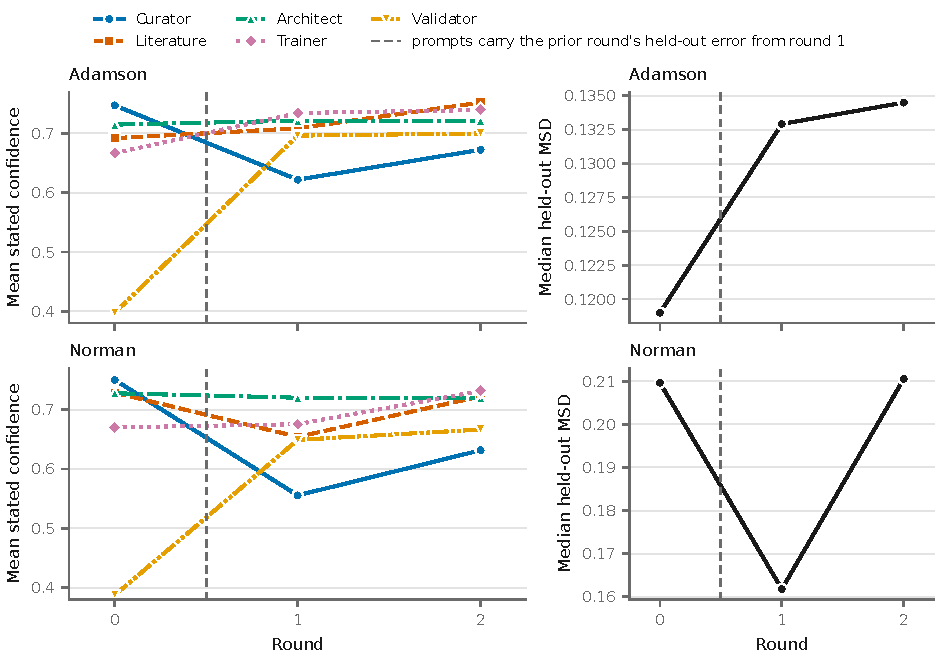
\includegraphics[width=\linewidth]{figures/fig_confidence_by_round.pdf}
\caption{Stated confidence and held-out error by round, for the Adamson tasks (top row) and
the Norman tasks (bottom row); rounds are numbered from $0$. The left panels show the mean
stated confidence of each of the five roles, where the value for a task is the median over its
three seeds and the mean is taken over tasks; the legend's Curator is the DataCurator role.
The right panels show the median over tasks of the held-out error, the mean squared deviation
(MSD) on the evaluation genes. The dashed vertical line marks the point from which every prompt
carries the previous round's held-out error. The figure is exploratory and was added after the
outcome was known.}
\label{fig:conf-by-round}
\end{figure}

\begin{figure}[htp]
\centering
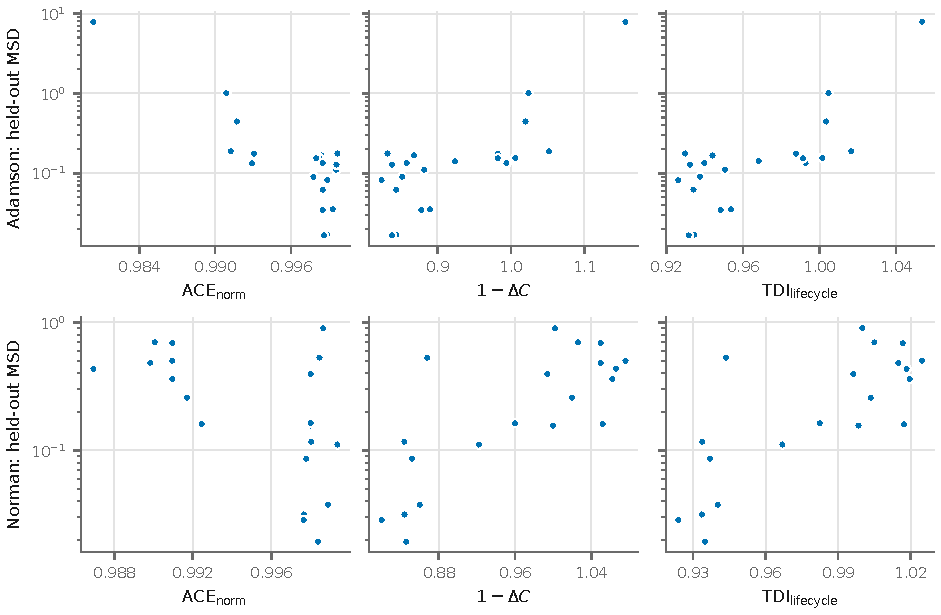
\includegraphics[width=\linewidth]{figures/fig_h4_scatter.pdf}
\caption{The data behind the six pre-registered tests of Table~\ref{tab:tdi-real}, for the
Adamson tasks (top row) and the Norman tasks (bottom row), with one point per task. The
vertical axis is the held-out error, the mean squared deviation (MSD) on the evaluation genes,
on a logarithmic scale. The horizontal axes are the three trace features:
$\mathrm{ACE}_{\mathrm{norm}}$, the normalised entropy of the agents' final-round confidences;
$1-\Delta C$, one minus the change in their mean confidence from the first round to the last;
and $\mathrm{TDI}_{\mathrm{lifecycle}}$, the weighted composite of the two
(\S\ref{sec:tdi-real}). Every value is the median over the three seeds of a task. No fitted
line or statistic is drawn; Spearman's rank correlations $\rho$ are those of
Table~\ref{tab:tdi-real}. The figure was added after the outcome was known, under the sixth
amendment to the pre-registration (Table~\ref{tab:amendments}).}
\label{fig:h4-scatter}
\end{figure}

\paragraph{Before feedback, mean confidence does not rank tasks.} The mean confidence stated in
round $0$ has no detectable rank association with the final error in either screen
($\rho=\explAdaConfRZeroMsdRho$ on Adamson and $\explNorConfRZeroMsdRho$ on Norman; both intervals
include zero), and it hardly varies across tasks: its standard deviation across tasks is
\explAdaConfSdRZero{} on Adamson and \explNorConfSdRZero{} on Norman, against \explAdaConfSdRTwo{}
and \explNorConfSdRTwo{} in round $2$.

\paragraph{After feedback, it does.} The mean confidence of rounds $1$ and $2$ is strongly and
negatively rank-associated with the final error, and $1-\Delta C$ is associated with the errors
the agents had been shown about as strongly as with the final error it was tested against. The
rank order of tasks by error is close to a property of the task: it barely changes from round to
round, and the lifecycle's final MSD ranks tasks almost as the trainer sweep's oracle does
(Table~\ref{tab:exploratory}). The rank order of tasks by the difficulty proxy thus depends
little on the agents' choices. Its level does depend on them: the lifecycle's percentile rank
within the trainer sweep differs between the screens (a median of \explAdaOraclePctRankMedian{}
on Adamson and \explNorOraclePctRankMedian{} on Norman; see the paragraph ``Stability and the
sweep'' at the end of this subsection). Read with
the design, the pre-registered pass is consistent with \emph{stated confidence falling further
on tasks where the agents were shown a larger held-out error}; it is not evidence that the
group's confidence anticipates difficulty before any error is measured. Nor does it isolate the
error as the cause, because the prompts of rounds $1$ and $2$ carry more than the error
(\S\ref{sec:limits}).

\paragraph{Which role moves.} The change in mean confidence from round $0$ to round $2$ is not
shared evenly (Figure~\ref{fig:conf-by-round}). The Validator, the only role on the larger
model, states a low confidence in round $0$ and a much higher one afterwards
(\explAdaRoleValidatorConfChange{} on Adamson and \explNorRoleValidatorConfChange{} on Norman), the
DataCurator's falls (\explAdaRoleCuratorConfChange{} and \explNorRoleCuratorConfChange), and the
Architect's barely moves (\explAdaRoleArchitectConfChange{} and \explNorRoleArchitectConfChange).
Role is confounded with model for the Validator.

\paragraph{One pre-feedback association, reported and not claimed.} On Norman the round-$0$
$\mathrm{ACE}_{\mathrm{norm}}$ is negatively associated with the final error
($\rho=\explNorAceRZeroMsdRho$, interval excluding zero); on Adamson the estimate has the same sign
and its interval includes zero ($\explAdaAceRZeroMsdRho$). This is one of \explNCorrelations{}
unplanned correlations, in the direction opposite to the pre-registered one, and it generates no
claim; testing it needs a new pre-registration.

\paragraph{Stability and the sweep.} When one task at a time is left out, the pre-registered
$1-\Delta C$ correlation ranges over [\explAdaLotoDcRhoMin, \explAdaLotoDcRhoMax] on Adamson and
[\explNorLotoDcRhoMin, \explNorLotoDcRhoMax] on Norman; the criterion is evaluated once, on all
tasks, and this range re-decides nothing. Within each task's \resNTrainerRecordsPerTask{} trainer
records, the lifecycle's final MSD sits at a median percentile rank of \explAdaOraclePctRankMedian{}
on Adamson and \explNorOraclePctRankMedian{} on Norman (lower is better). The comparison is
descriptive: the lifecycle's applied hyperparameters are not on the trainer grid.

\subsection{Run record}\label{subsec:runrecord}

The sweep was a single run, identified with its code revision and manifest in
\S\ref{sec:reproducibility}. It analysed \resNTasks{} tasks with \resNLifecycleRuns{} lifecycle
runs, each of exactly three rounds, comprising \resNSteps{} agent steps, all LLM-sourced. A
valid run admits no step from the rule-based fallback, from a mock or from an unknown source,
and the counts of such steps are \resNFallback, \resNStepsMock{} and \resNStepsUnknown. The LLM
cache held \resCacheStart{} entries at the start, there were \resCacheHits{} cache hits, and
no reply was replayed from the cache (the recorded replay flag is \resReplay). Of the
\resNCalls{} API calls, \resStopEndTurn{} ended normally, and those that reached their output
ceiling (\resStopMaxTokens) were each retried once at twice the ceiling and then answered. There were \resRefusals{} refusals and \resServedMismatch{} calls whose served model
differed from the requested one, and the calls used \resTokensIn{} input and \resTokensOut{}
output tokens. The DataCurator, Literature, Architect and Trainer roles were served by
Claude Haiku 4.5, \resRoleServedCurator{} (\resRoleCallsCurator, \resRoleCallsLiterature, \resRoleCallsArchitect{}
and \resRoleCallsTrainer{} calls respectively), and the Validator by Claude Sonnet 5.5,
\resRoleServedValidator{}
(\resRoleCallsValidator{} calls), with \resNFailover{} failovers. Prices, in US dollars per
million input and output tokens, were \resPriceHaikuIn{} and \resPriceHaikuOut{} for Haiku and
\resPriceSonnetIn{} and \resPriceSonnetOut{} for Sonnet, with cache reads and writes at the
pinned multipliers. The preflight check found \resLivenessOkPairs{} of \resLivenessTotalPairs{}
model--role probes live. The trainer sweep wrote \resNTrainerRuns{} records
(\resNTrainerRecordsPerTask{} per task).

Spend was \$\resSpendLLM{} on LLM calls (Haiku \$\resSpendHaiku{} and Sonnet \$\resSpendSonnet{}
in the sweep, plus \$\resSpendPreflight{} of preflight probes), \$\resSpendGPU{} on GPU time
(\resGPUHours{} A100-hours) and \$\resSpendPrior{} carried in from an earlier attempt at the sweep that was aborted and from the dry run, a total of
\$\resSpendTotal{} against a \$\resSpendStopLine{} stop-and-report line and a \$\resKillLine{}
kill line. Neither line was reached (recorded stop reason: \resStopReasonNone).

After the run, on \resRROneDate, the record of where the LLM API key was stored (no secret
value) was removed from \resRROneFileCount{} run files, the run manifest among them, because it
supports no claim. The manifest's SHA-256 prefix changed from \resManifestShaSuperseded{} to
\resManifestSha; no result changed (Appendix~\ref{app:rr}).
